\documentclass{article}

\usepackage{graphicx}
\usepackage{tikz}
\usepackage{tikzsymbols}
\usetikzlibrary{calc,patterns,shapes.geometric}
\pagestyle{empty}
\usepackage[margin=0pt]{geometry}
\geometry{papersize={14in,12in}}

\def\centerarc[#1](#2)(#3:#4:#5){\draw[#1] ($(#2)+({#5*cos(#3)},{#5*sin(#3)})$) arc (#3:#4:#5);}

\begin{document}
	\begin{figure}
		\centering
		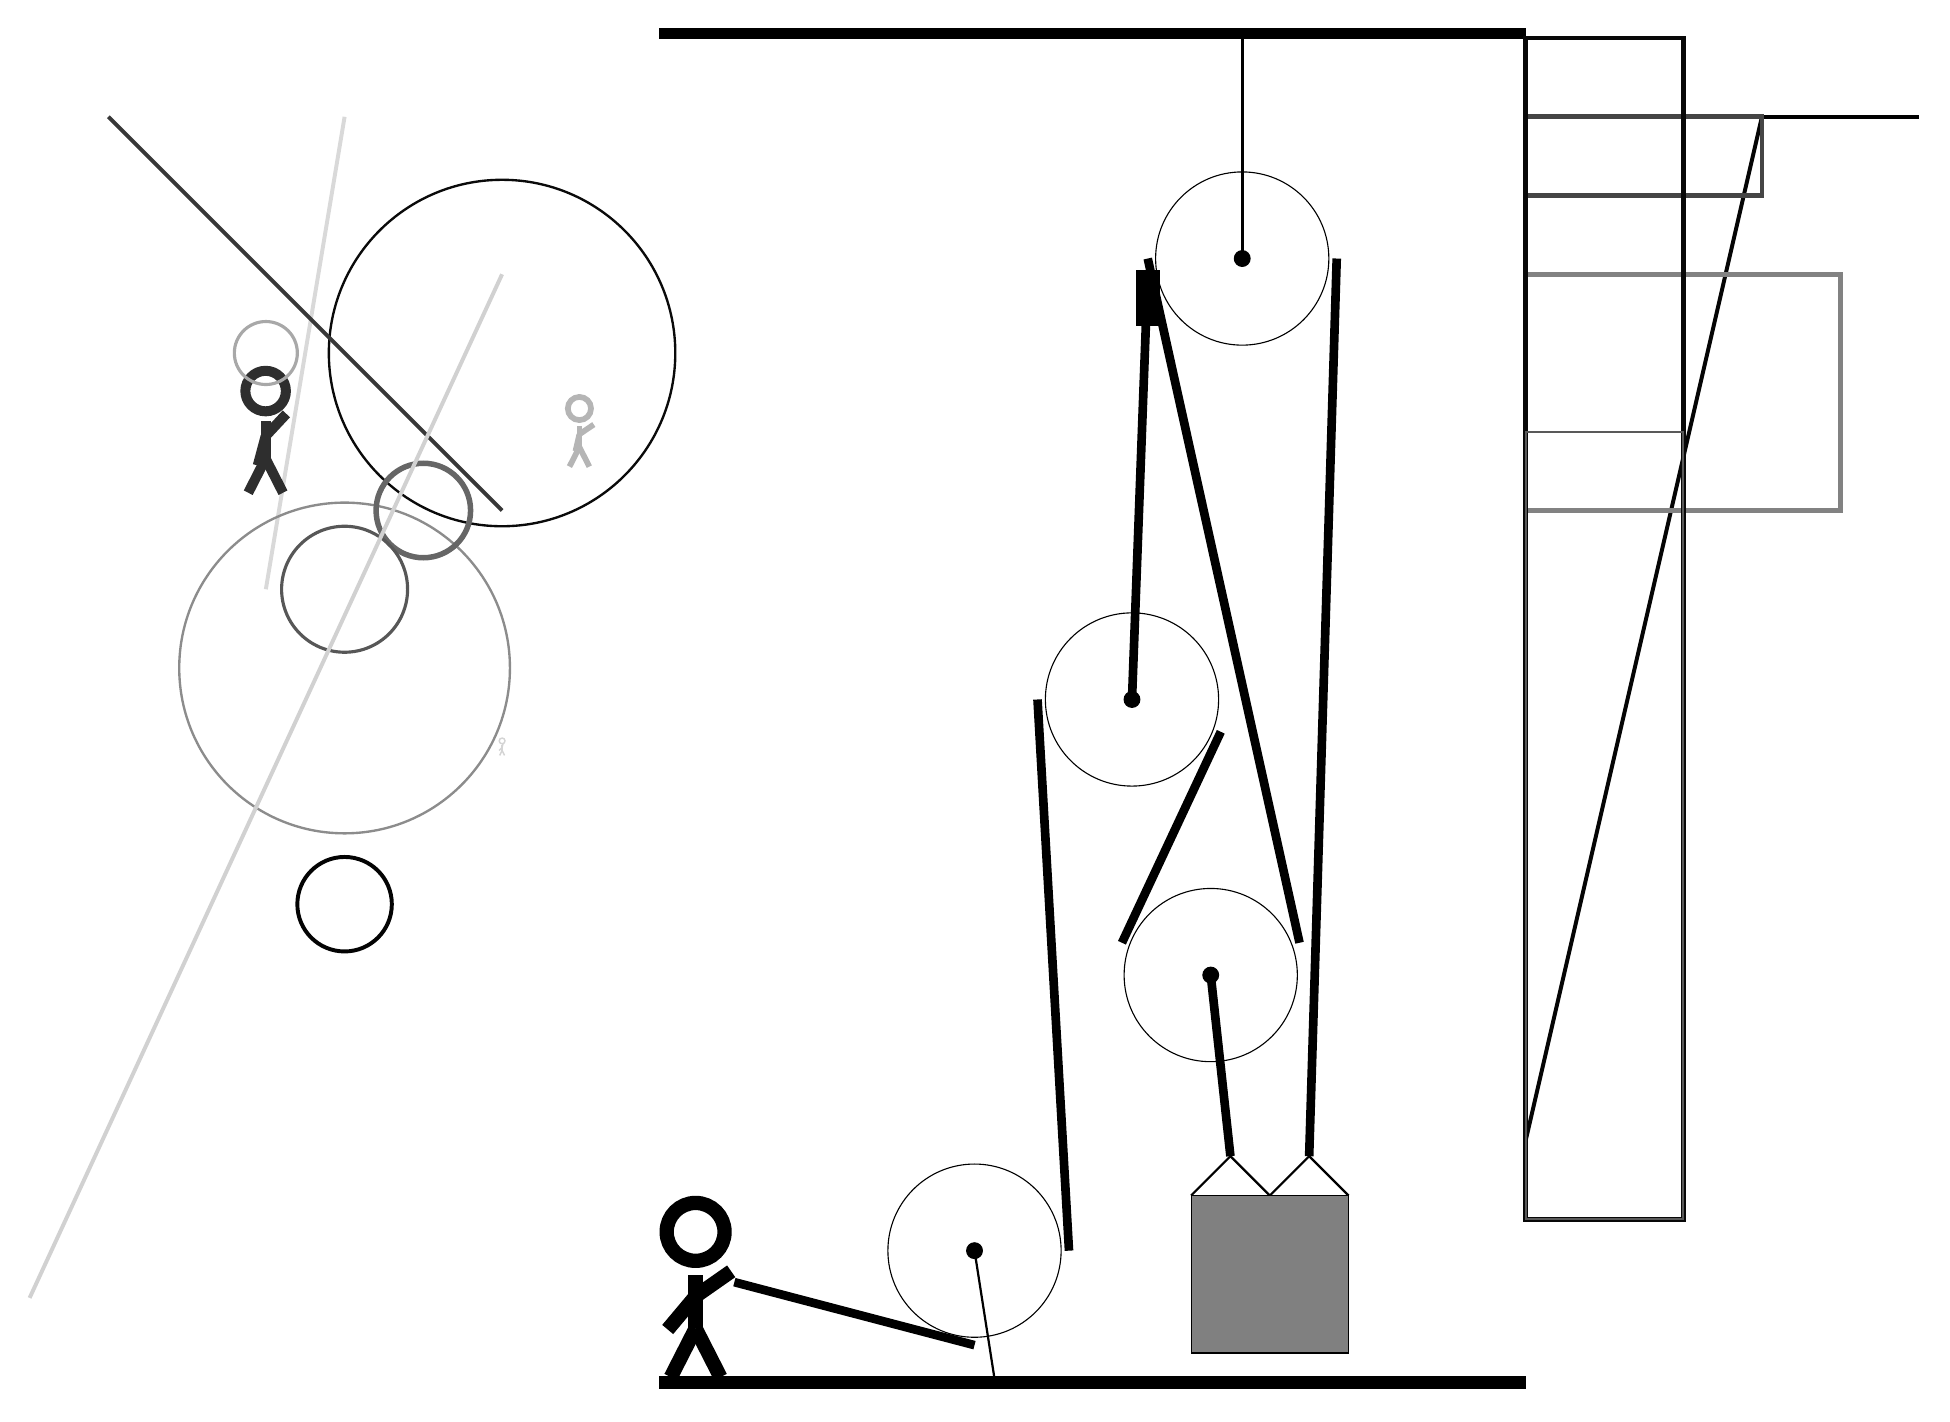
\begin{tikzpicture}
			%%%%% START %%%%%
			
			\draw[fill=black] (-6, 14) rectangle (5, 14.125);
			
			\draw (0, 5.6) circle (1.1);
			\draw[fill=black] (0, 5.6) circle (0.1);
			
			\draw (1, 2.1) circle (1.1);
			\draw[fill=black] (1, 2.1) circle (0.1);
			
			\draw (1.4, 11.2) circle (1.1);
			\draw[fill=black] (1.4, 11.2) circle (0.1);
			\draw[very thick] (1.4, 11.2) -- (1.4, 14);
			
			\draw (-2, -1.4) circle (1.1);
			\draw[fill=black] (-2, -1.4) circle (0.1);
			\draw[thick] (-2, -1.4) -- (-1.75, -3);
			
			
			\draw[thick]  (0.75, -0.7) -- (1.25, -0.2) -- (1.75, -0.7) -- (2.25, -0.2) -- (2.75, -0.7);
			\draw[fill=black!50] (0.75, -0.7) rectangle (2.75, -2.7);
			\draw[line width=1.1mm] (-5.05, -1.8) -- (-2, -2.6);
			\centerarc[line width=1.1mm](-2, -1.4)(270:360:1.2000000000000002);
			\draw[line width=1.1mm] (-0.8, -1.4) -- (-1.2, 5.6);
			\draw[line width=1.1mm] (0, 5.6) -- (0.2, 11.0);
			\draw[line width=1.1mm, fill=black](0.1, 10.4) rectangle (0.3, 11.0);
			\centerarc[line width=1.1mm](0, 5.6)(-20:180:1.2000000000000002);
			\draw[line width=1.1mm] (1.1276, 5.1896) -- (-0.1276, 2.5104);
			\centerarc[line width=1.1mm](1, 2.1)(160:380:1.2000000000000002);
			\draw[line width=1.1mm] (2.1276, 2.5104) -- (0.2, 11.2);
			\draw[line width=1.1mm](1, 2.1) -- (1.25, -0.2);
			\centerarc[line width=1.1mm](1.4, 11.2)(0:180:1.2000000000000002);
			\draw[line width=1.1mm] (2.6, 11.2) -- (2.25, -0.2);
			
			\draw[line width=0.5mm, color=black!15](-10, 13) -- (-11, 7);
			
			\node[line width=0.6mm, color=black!82] at (-11, 9) {\Strichmaxerl[7][75][47]};
			\draw[line width=0.5mm, color=black!100](7, 13) -- (10, 13);
			\draw [line width=0.3mm, color=black!96](-8, 10) circle (2.2);
			\node[line width=0.2mm, color=black!17] at (-8, 5) {\Strichmaxerl[1][47][76]};
			\draw[line width=0.5mm, color=black!78](-8, 8) -- (-13, 13);
			\draw [line width=0.3mm, color=black!45](-10, 6) circle (2.1);
			\draw [line width=0.5mm, color=black!99](-10, 3) circle (0.6);
			\draw [line width=0.7mm, color=black!60](-9, 8) circle (0.6);
			\draw [line width=0.4mm, color=black!66](-10, 7) circle (0.8);
			\draw[line width=0.5mm, color=black!98](8, 13) -- (5, 0);
			
			\draw[line width=0.5mm, color=black!18](-8, 11) -- (-14, -2);
			\draw[line width=0.6mm, color=black!73] (5, 13) rectangle (8, 12);
			
			\node[line width=0.4mm, color=black!29] at (-7, 9) {\Strichmaxerl[4][77][34]};
			\draw [line width=0.4mm, color=black!34](-11, 10) circle (0.4);
			\draw[line width=0.7mm, color=black!49] (5, 8) rectangle (9, 11);
			
			\draw[line width=0.6mm, color=black!97] (5, -1) rectangle (7, 14);
			\draw[line width=0.3mm, color=black!65] (5, -1) rectangle (7, 9);
			
			\node at (-5.5, -1.9) {\Strichmaxerl[10][50][35]};
			
			\draw[fill=black] (-6, -3) rectangle (5, -3.15);
			
			%%%%% END %%%%%
		\end{tikzpicture}
	\end{figure}	
\end{document}